\documentclass{beamer}
%\usepackage[all,arc,curve,frame,color]{xy}
%\usepackage{tkz-graph}
\usepackage{mathtools}
\usepackage{ragged2e,etoolbox}


\newenvironment{nstabbing}
  {\setlength{\topsep}{0pt}%
   \setlength{\partopsep}{0pt}%
   \tabbing}
  {\endtabbing}

\def\jump{ \quad \\ \vspace{0.5cm} \pause}
\newcommand{\nc}{\newcommand}
\nc{\pid}{\mathfrak{p} }
\nc{\dpid}{\delta_{\mathfrak{p}}}

\def\AA{{\mathbb A}}
\def\CC{{\mathbb C}}
\def\EE{{\mathcal E}}
\def\FF{{\mathcal F}}
\def\GG{{\mathcal G}}
\def\HH{{\mathcal H}}
\def\MM{{\mathcal M}}
\def\NN{{\mathbb N}}
\def\PP{{\mathbb P}}
\def\QQ{{\mathbb Q}}
\def\RR{{\mathbb R}}
\def\ZZ{{\mathbb Z}}
\def\aa{{\mathbf a}}
\def\bb{{\mathbf b}}
\def\del{\partial}
\def\kk{\Bbbk}
\def\mm{{\mathfrak m}}
\def\nn{{\mathfrak n}}
\def\pp{{\mathfrak p}}
\def\qq{{\mathfrak q}}
\def\rr{{\mathbf r}}
\def\uu{{\mathbf u}}
\def\vv{{\mathbf v}}
\def\ww{{\mathbf w}}
\def\xx{{\mathbf x}}
\def\yy{{\mathbf y}}
\def\zz{{\mathbf z}}
\newcommand{\PGL}{\textrm{PGL}}
\newcommand{\res}{\textrm{Res}}


\DeclareMathOperator{\Tail}{Tail}
\DeclareMathOperator{\Per}{Per}
\DeclareMathOperator{\PrePer}{PrePer}

\makeatletter
\def\th@mystyle{%
    \normalfont % body font
    \setbeamercolor{block title example}{bg=orange,fg=white}
    \setbeamercolor{block body example}{bg=orange!20,fg=black}
    \def\inserttheoremblockenv{exampleblock}
  }
\makeatother

\makeatletter
\def\th@thmstyle{%
    \normalfont % body font
    \setbeamercolor{block title example}{bg=blue,fg=white}
    \setbeamercolor{block body example}{bg=blue!20,fg=black}
    \def\inserttheoremblockenv{exampleblock}
  }
\makeatother

\definecolor{darkgreen}{RGB}{77,153,0}
\makeatletter
\def\th@qstnstyle{%
    \normalfont % body font
    \setbeamercolor{block title example}{bg=darkgreen,fg=white}
    \setbeamercolor{block body example}{bg=green!20,fg=black}
    \def\inserttheoremblockenv{exampleblock}
  }
\makeatother


\theoremstyle{thmstyle}
\newtheorem*{mythm}{Theorem}

\theoremstyle{mystyle}
\newtheorem*{remark}{Remark}
\newtheorem*{conjecture}{Conjecture}
\newtheorem*{mycor}{Corollary}
\newtheorem*{mylemma}{Lemma}

\theoremstyle{qstnstyle}
\newtheorem*{question}{Question}

\usepackage{remreset}% tiny package containing just the \@removefromreset command
\makeatletter
\@removefromreset{subsection}{section}
\makeatother
\setcounter{subsection}{1}

\newcommand\Wider[2][3em]{%
\makebox[\linewidth][c]{%
  \begin{minipage}{\dimexpr\textwidth+#1\relax}
  \raggedright#2
  \end{minipage}%
  }%
}

\mode<presentation>{\usetheme{CambridgeUS}\usecolortheme{dolphin}} 
%\setbeamertemplate{navigation symbols}{}
\setbeamertemplate{blocks}[rounded][shadow=false]


\title[Bounds for preperiodic points]{Scarcity of finite orbits for rational functions over a number fields. }
%\subtitle{long subtitle}
\author[Sebastian Troncoso]{Sebastian Troncoso}
\institute[BSC]{Birmingham-Southern College\\ \vspace{5mm} Spring Southeastern Sectional Meeting \\ Vanderbilt University, Nashville, TN}
%\titlegraphic{\includegraphics[height=1.5cm]{../images/normale_pisa.png}}
\date[ April 15, 2018.]{ April 15, 2018. \\ \vspace{1cm} }


%\AtBeginSection[]{} % for optional outline or other recurrent slide
\AtBeginSection{\frame{\sectionpage}}
\begin{document}

\begin{frame}
\titlepage
\end{frame}

\begin{frame}
\frametitle{Notation}
%Let $K$ be a number field and $\mathcal{O}_K$ its ring of algebraic integers,
%\jump
Let $\phi:\mathbb{P}^n\to\mathbb{P}^n$ be an endomorphism defined over a number field $K$.
\jump
\textbf{Periodic point}: $\phi^m(P)=P$ for some $m\geq{1}$.
% Minimal $n$ is called the \textbf{period} of $P$.
%The set of $K$-rational periodic points is denoted by $Per(\phi,K)$.

\jump
\textbf{Preperiodic point}: $\exists m\geq{0}$ such that $\phi^m(P)$ is periodic.\\ 
%i.e. $P$ has finite orbit. \\ 
The set of $K$-rational preperiodic points is denoted by $PrePer(\phi,K)$.

\jump
\textbf{Tail point}: A point that is preperiodic but not periodic.\\ 
%The set of $K$-rational tail points is denoted by $Tail(\phi,K)$.

\end{frame}

\begin{frame}
\frametitle{Examples:}
We can view $\mathbb{P}^1(K)$ as $K\cup\infty$ and endomorphism of $\PP^1$ as rational functions.
\begin{center}
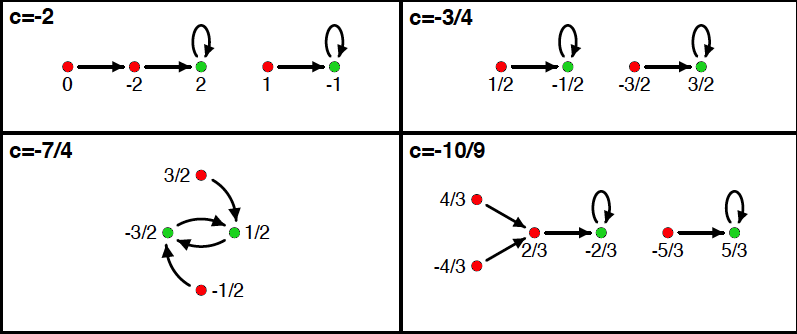
\includegraphics[width=1.0\linewidth]{placeholder4}
\end{center}

$\QQ$-rational tail points (red) and $\QQ$-rational periodic points (green) of  $\phi_c(z)=z^2+c$.
\end{frame}

\begin{frame}
\frametitle{Question:}
\begin{itemize}
\item Is the set $\PrePer(\phi,K)$ finite? 

\pause \textbf{Yes}. 
\vspace{6mm}\pause

\begin{mythm}[Northcott 1950]
Let $\phi : \PP^n \to \PP^n$ be an endomorphism of degree $\geq{2}$
defined over a number field $K$. Then $\phi$ has
only finitely many preperiodic points in $\PP^n(K)$.
\end{mythm}


\pause \vspace{3mm}
\end{itemize}
\begin{itemize}
\item How large is the set $\PrePer(\phi,K)$? 
\item Can we give an explicit bound?
\item How is the bound depending on $\phi$? 

\end{itemize}

\end{frame}


\begin{frame}
We can deduce from the original proof of Northcott's theorem  a bound for $|\PrePer(\phi,K)|$ depending on
\begin{itemize}
\item  $D=[K: \QQ]$ 

\item The dimension $n$ of the projective space  

\item The degree $d$ of $\phi$.

\item height of the coefficients of $\phi$
\end{itemize}

\end{frame}

\begin{frame}
\frametitle{Example}
Consider $f(x)=(x-1)(x-2)(x-3)\ldots(x-d)+x$.
\pause

Notice that $f$ has at least $d$ periodic points. 
$$1 \circlearrowleft  $$
$$2 \circlearrowleft  $$
$$\vdots  $$
$$d \circlearrowleft  $$

\pause

\end{frame}





\begin{frame}
\frametitle{The Dream:}
Give explicit bounds for $|\PrePer(\phi,K)|$ in terms of:\pause
\begin{itemize}

\item  $D=[K: \QQ]$ 

\item The dimension $n$ of the projective space 

\item The degree $d$ of $\phi$.
\end{itemize}

\pause

\begin{conjecture}[Uniform Boundedness Conjecture - Morton--Silverman
  1994]
There exists a bound $B = B(D,n,d)$ such that if $K/\mathbb{Q}$ is a number field of degree $D$, and $\phi:\mathbb{P}^n\rightarrow\mathbb{P}^n$ is an endomorphism of degree $d\geq{2}$ defined over $K$, then 
$$|\text{PrePer}(\phi,K)| \leq B.$$
\end{conjecture}
\end{frame}


%\begin{frame}
%\frametitle{Uniform boundedness of preperiodic points}
%\begin{mythm}[Northcott 1950]
%Let $\phi : \PP^n \to \PP^n$ be a morphism of degree $\geq{2}$
%defined over a number field $K$. Then $\phi$ has
%only finitely many preperiodic points in $\PP^n(K)$.
%\end{mythm}
%
%\quad\\
%
%\pause
%
%\begin{conjecture}[Uniform Boundedness Conjecture - Morton--Silverman
%  1994]
%There exists a bound $B = B(D,n,d)$ such that if $K/\mathbb{Q}$ is a number field of degree $D$, and $\phi:\mathbb{P}^n\rightarrow\mathbb{P}^n$ is a morphism of degree $d\geq{2}$ defined over $K$, then 
%$$\#\text{PrePer}(\phi,K) \leq B.$$
%%the number of $K$-preperiodic points of $f$ is less than or equal to $B$.
%\end{conjecture}
%
%\end{frame}


\begin{frame}
\frametitle{Goal:}

\begin{itemize}


\item Give an explicit bound for $|\PrePer(\phi,K)|$.

\vspace{10mm} 

\item To do so we need an extra parameter. 

\vspace{10mm} 

\item Instead of the height of $\phi$ we use a weaker and more natural parameter.
\vspace{10mm} 



\item This parameter is the number of places of bad reduction of $\phi$

\end{itemize}


\end{frame}

\begin{frame}
\frametitle{Good reduction}

\begin{itemize}
\item For simplicity in the notation we will defined good reduction only for rational maps $\phi:\mathbb{P}^1\to\mathbb{P}^1$. \pause
\item Let $K$ be a number field, $\mathcal{O}_K$ its ring of algebraic integers, $\mathfrak{p}$ a non zero prime ideal of $\mathcal{O}_K$
and $\mathcal{O}_{\mathfrak{p}}$ the local ring at $\pid$. \pause
\item Write $\phi$ in normal form: 
$$\phi([x : y]) = [F(x, y): G(x, y)],$$
where $F(x, y)$ and $G(x, y)$ are coprime
homogeneous polynomials of the same degree, with coefficients in $\mathcal{O}_\pid$ and at least one a $\pid$-unit. \pause
\item We say $\phi$ has \textbf{good reduction} at $\pid$ if $F$ and $G$ do not have a common zero module $\pid$ in $\mathbb{P}^1$.   

%\pause
%\item By convention, we say $\phi$ has bad reduction at all archimedean places.
\end{itemize}
\end{frame}

%\begin{frame}
%\frametitle{Bound on maximal period}
%\begin{mythm}[W.\ Narkiewicz 1988]
%Let $\phi \in K[z]$ be a polynomial of degree $\geq{2}$
%defined over a number field $K$ of degree $D=[K:\QQ]$. 
%Suppose $\phi$ has good reduction outside a finite set of places $S$, including all archimedean ones. Let $s=|S|$.
%\\\quad\\
%If $P$ is a $K$-rational periodic point of period $n$, then
%$$ n \leq (6\cdot 7^{D+2s})^\alpha,$$ where $\alpha=O(s\log{s}).$
%\end{mythm}
%\end{frame}




%\begin{frame}
%\frametitle{Bound on maximal orbit length of a preperiodic point}
%\begin{mythm}[J.K.\ Canci 2006]
%Let $\phi : \PP^1\to\PP^1$ be a rational map of degree at least two
%defined over a number field $K$. 
%Suppose $\phi$ has good reduction outside a finite set of places $S$, including all archimedean ones. Let $s=|S|$.
%\\\quad\\
%If $P\in\text{PrePer}(\phi,K)$ is of orbit length $n$, then
%$$n\leq\left[{e^{10}}^{12}(s+1)^8(log(5(s+1)))^8\right]^s.$$
%\end{mythm}
%\end{frame}

\begin{frame}
\frametitle{Bound on the set of preperiodic point for a rational map} 
\begin{mythm}


Let $\phi : \PP^1\to\PP^1$ be a rational map of degree $d\geq{2}$
defined over a number field $K$ and $[K: \mathbb{Q}]=D$. 
Suppose $\phi$ has good reduction outside a finite set of places $S$, including all archimedean ones. Let $s=|S|$. Then \pause
\begin{itemize}
%d^{ \max\left\{(2^{16s-8}+3)\left[12s\log(5s)\right]^{D}, \left[12(s+2)\log(5s+5)\right]^{4D}\right\}}

\item $|PrePer(K,\phi)|\leq  d^{2^{16s}\left(s\log(s)\right)^D}$
 \\ J.K.\ Canci and L.\ Paladino (2015).\jump
\item $|PrePer(K,\phi)|\leq 5\left(2^{16sd^3}\right)+3$
 \\ S.\ Troncoso (2017).\jump
\item $|PrePer(K,\phi)|\leq \alpha d^2+\beta d+\gamma$ \\  where $\alpha$, $\beta$ and $\gamma$ are roughly $2^{78s}$.
\\ J.K.\ Canci, S.\ Troncoso and S.\ Vishkautsan (submitted).

\end{itemize}
\end{mythm}
\end{frame}

%\begin{frame}
%\frametitle{Reciprocity of periodic and tail points}
%\begin{mythm}[S.\ Troncoso 2016]
%Let $\phi$ be an endomorphism of $\PP^1$, defined over $K$. Suppose $\phi$ has good reduction outside $S$. Let $R\in\PP^1(K)$ be a tail point and let $n$ be the period of the periodic part of the orbit of $R$. Let $P\in\PP^1(K)$ be any periodic point that is not $\phi^{mn}(R)$ for some $m$. Then $\delta_\pp(P,R)=0$ for every $\pp \notin S$.
%\end{mythm}
%\end{frame}

%\begin{frame}
%\frametitle{Techniques}
%\begin{itemize}
%\item The $\pp$-adic logarithmic distance of almost every pair of $K$-rational tail point and $K$-rational periodic point is $0$. \pause \\ There is a strong arithmetic relation between periodic and tail points.
%\jump
%\item Explicit bounds for the number of solutions of the $S$-unit equation. \pause That means a linear relations of the form $$u+v=1$$  where  $(u,v) \in \left(\mathcal{O}_S^*\right)^2$.
%% and $a,b\in{K}$. ($\mathcal{O}_S^{*}$ is the group of $S$-units) \pause
%%\item Beukers and Schlickewei's explicit bound on the number of solutions $(u,v) \in \left(\mathcal{O}_S^{*}\right)^2$ to the $S$-unit equation.\pause For $a,b\in{K}$ the number of solutions of $$au+bv=1$$ is bounded by $$2^{8(2|S|+2)}$$ \pause
%%\item The finitely many solutions to $au+bv=1$ give us a bound on $Per(\phi,K)$, $Tail(\phi,K)$ and $PrePer(\phi,K)$. 
%\end{itemize}
%\end{frame}

\begin{frame}
\frametitle{Tools}
\begin{itemize}
\item Logarithmic $v$-adic distance between points in $\PP^1(K)$.

\begin{center}
{\huge{$\downarrow$}}
\end{center}
\pause
\item Study the distance between tail point and periodic.

\begin{center}
{\huge{$\downarrow$}}
\end{center}
\pause
\item The set of tail points and the set of periodic points bound each other.

\begin{center}
{\huge{$\downarrow$}}
\end{center}
\pause
\item Number of solution of the $S$-unit equation.
\begin{center}
{\huge{$\downarrow$}}
\end{center}
\pause
\item Get a bound for the set of preperiodic point under a mild hypothesis
\begin{center}
{\huge{$\downarrow$}}
\end{center}
\pause
\item We use big theorems to lift the mild hypothesis and get the theorem. \\ (Riemann-Hurwitz, Baker's Theorem, Kisaka's analysis on Baker's Theorem)


\end{itemize}
\end{frame}

\begin{frame}
\begin{center}
{\Huge{THANK YOU}}
\end{center}


\end{frame}


\end{document}